\documentclass[a4paper,11pt]{article}
\input{/home/tof/Documents/Cozy/latex-include/preambule_lua.tex}
\newcommand{\showprof}{show them}  % comment this line if you don't want to see todo environment
\fancyhead[L]{Exercices arbre binaire}
\newdate{madate}{10}{09}{2020}
%\fancyhead[R]{\displaydate{madate}} %\today
%\fancyhead[R]{Seconde - SNT}
%\fancyhead[R]{Première - NSI}
\fancyhead[R]{Terminale - NSI}
\fancyfoot[L]{~\\Christophe Viroulaud}
\AtEndDocument{\label{lastpage}}
\fancyfoot[C]{\textbf{Page \thepage/\pageref{lastpage}}}
\fancyfoot[R]{\includegraphics[width=2cm,align=t]{/home/tof/Documents/Cozy/latex-include/cc.png}}
\usepackage{tikz}

\begin{document}
\begin{Form}
\begin{exo}
\begin{enumerate}
\item \begin{itemize}
\item préfixe: × - 12 8 + 7 9
\item infixe: 12 - 8 × 7 + 9
\item postfixe: 12 8 - 7 9 + ×
\end{itemize}
\item 64
\item Parcours infixe
\end{enumerate}
\end{exo}
\begin{exo}
\begin{enumerate}
\item 
\begin{itemize}
\item en largeur: 1 2 3 4 5 6 7 8 9 10 11 12 13
\item préfixe: 1 2 4 8 5 3 6 9 10 12 13 7 11
\item infixe: 4 8 2 5 1 9 6 12 10 13 3 11 7
\item postfixe: 8 4 5 2 9 12 13 10 6 11 7 3 1
\end{itemize}
\item La hauteur est 4.
\item Cet arbre est équilibré car la hauteur de chaque sous-arbre gauche diffère au plus de 1 de chaque sous-arbre droit.
\item Cet arbre n'est pas complet car tous les niveaux ne sont pas remplis.
\end{enumerate}
\end{exo}
\begin{exo}
\begin{enumerate}
\item Le numéro 17 est une femme (indice impair). Son père a pour indice 34 et sa mère 35. Son enfant a pour indice 8.
\item Quatrième génération: $2^4 = 16$ personnes (la numérotation commence à 1).
\item Chaque niveau \emph{i} contient $2^{i-1}$ ascendants (la numérotation commence à 1). La somme de tous les niveaux correspond à la somme de termes d'une suite géométrique de raison 2 et de premier terme 1. $$2^0+2^1+2^2+2^3+2^4=\sum_{k=0}^{4}{2^k}=\dfrac{1-2^{4+1}}{1-2}=31$$
\item Représentation\\
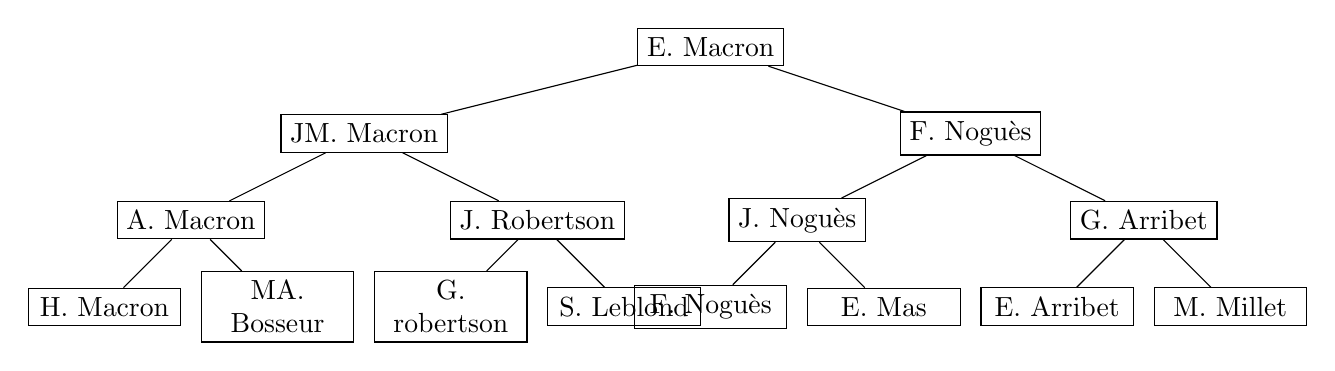
\begin{tikzpicture}[scale=1.1]
\node[draw] (A) at (1,0) {E. Macron};
\node[draw] (B) at (-3,-1) {JM. Macron};
\node[draw] (C) at (-5,-2) {A. Macron};
\node[draw] (D) at (-1,-2) {J. Robertson};
\node[draw,text width=1.7cm,text centered] (E) at (-6,-3) {H. Macron};
\node[draw,text width=1.7cm,text centered] (F) at (-4,-3) {MA. Bosseur};
\node[draw,text width=1.7cm,text centered] (H) at (-2,-3) {G. robertson};
\node[draw] (I) at (4,-1) {F. Noguès};
\node[draw] (J) at (2,-2) {J. Noguès};
\node[draw] (K) at (6,-2) {G. Arribet};
\node[draw,text width=1.7cm,text centered] (L) at (0,-3) {S. Leblond};
\node[draw,text width=1.7cm,text centered] (M) at (1,-3) {F. Noguès};
\node[draw,text width=1.7cm,text centered] (N) at (3,-3) {E. Mas};
\node[draw,text width=1.7cm,text centered] (O) at (5,-3) {E. Arribet};
\node[draw,text width=1.7cm,text centered] (P) at (7,-3) {M. Millet};

\draw (A) -- (B);
\draw (C) -- (B);
\draw (C) -- (E);
\draw (C) -- (F);
\draw (D) -- (B);
\draw (D) -- (H);
\draw (A) -- (I);
\draw (J) -- (I);
\draw (I) -- (K);
\draw (L) -- (D);
\draw (J) -- (M);
\draw (J) -- (N);
\draw (K) -- (O);
\draw (K) -- (P);
\end{tikzpicture}
\item Ouvrir le fichier \emph{arbre-genealogique.py}.
\item Les parents
\lstinputlisting[firstline=17,lastline=20]{"scripts/arbre-genealogique.py"}
\item Pour parcourir le sous-arbre gauche en premier il faut empiler d'abord l'indice impair.
\lstinputlisting[firstline=22,lastline=34]{"scripts/arbre-genealogique.py"}
\item Dans ce cas c'est l'indice pair qui est utilisé en premier dans les appels.
\lstinputlisting[firstline=36,lastline=44]{"scripts/arbre-genealogique.py"}
\end{enumerate}
\end{exo}
\begin{exo}
\begin{enumerate}
\item Class
\lstinputlisting[firstline=10,lastline=19]{"scripts/class-arbre.py"}
\item Insertion
\lstinputlisting[firstline=21,lastline=29]{"scripts/class-arbre.py"}
\item Création
\lstinputlisting[firstline=80,lastline=87]{"scripts/class-arbre.py"}
\item Préfixe
\lstinputlisting[firstline=31,lastline=38]{"scripts/class-arbre.py"}
\item Infixe et postfixe
\lstinputlisting[firstline=47,lastline=54]{"scripts/class-arbre.py"}
\lstinputlisting[firstline=63,lastline=70]{"scripts/class-arbre.py"}
\item Variante
\lstinputlisting[firstline=40,lastline=45]{"scripts/class-arbre.py"}
\end{enumerate}
\end{exo}
\end{Form}
\end{document}